\documentclass[titlepage,a4paper,12pt]{report}
\usepackage{amssymb,amsfonts,amsmath}
\usepackage{fullpage}
\usepackage{graphicx}
%\usepackage[cc]{titlepic}
\usepackage{amsthm}
\newtheorem{definition}{Definition}[section]
\newtheorem{example}{Example}[section]
\newtheorem{theorem}{Theorem}[section]
\newtheorem{exercise}{Exercise}[section]
\newtheorem{corollary}{Corollary}[section]
\newtheorem{proposition}{Proposition}[section]
\pdfpagewidth 8.5in
\pdfpageheight 11in
\setlength\topmargin{-0.5in}
\setlength\headheight{0in}
\setlength\headsep{0in}
\setlength\textheight{9.5in}
\setlength\textwidth{7.0in}
\setlength\oddsidemargin{-0.5in}
\setlength\evensidemargin{1.0in}
\setlength\parindent{0.25in}
\setlength\parskip{0.25in}
%\begin{titlepage}
%\usepackage{titlepic}
%\titlepic{
\includegraphics[width=0.2\textwidth]{uz1.png}}
%
%\title{\textbf{HMTH111 Calculus 2}}
%\author{Nhawu. G\\
%		Department of Mathematics\\
%		University of Zimbabwe, ZIM}
%
%\end{titlepage}

\begin{document}
\begin{titlepage}
 
\begin{center}
 
 
% Upper part of the page

\includegraphics[width=0.15\textwidth]{uz1.png}\\[1cm]
 
\textsc{\LARGE University of Zimbabwe}\\[1.5cm]
 
\textsc{\Large HMTHCS111 CALCULUS 2}\\[0.5cm]
 
 
% Title

{ \huge \bfseries Calculus of Several Variables}\\[0.4cm]
 

 
% Author and supervisor
\begin{minipage}{0.4\textwidth}
\begin{center} \large
\emph{Author:}\\
G. \textsc{Nhawu}
\end{center}
\end{minipage}
\begin{minipage}{0.4\textwidth}
\begin{flushright} \large
\emph{Department:} \\
\textsc{Mathematics and Computational Sciences}
\end{flushright}
\end{minipage}

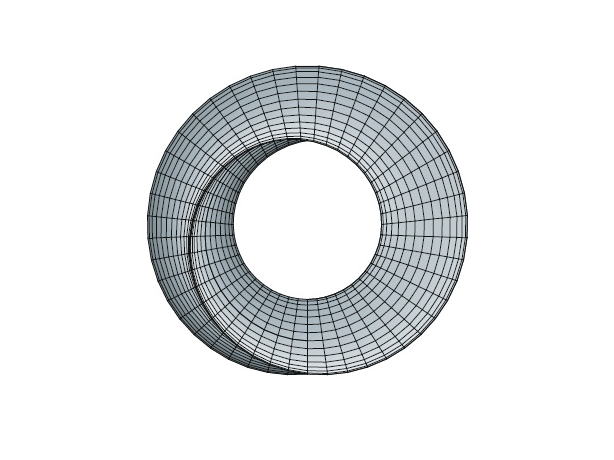
\includegraphics[width=0.7\textwidth]{umblictorus.png}\\[1cm]
 \vfill
 
 
% Bottom of the page
{\large \today}
 
\end{center}
 
\end{titlepage}
%\maketitle
\tableofcontents
\setcounter{chapter}{3}
\chapter{Coordinate Geometry in $3$ Dimensions}\begin{center}
\small{\parbox{18cm}{
		\begin{raggedright}
		{\small
		\textit{Every heart sings a song, incomplete, until another heart whispers back. Those who wish to sing always find a song. At the touch of a lover, everyone becomes a poet.}
 }
 
				\vspace{.5cm}\hfill{--- Plato}
		\end{raggedright}
	}
} 
\end{center}
A coordinate system represents a point in the plane by an ordered pair of numbers called
coordinates. Usually we use Cartesian coordinates, which are directed distances from two
perpendicular axes. Here we describe a coordinate system introduced by Newton, called
the \textbf{polar coordinate system}, which is more convenient for many purposes.

\noindent So far, we have been representing graphs as collections of points $(x,y)$ in the rectangular coordinate system. 
\section{Polar Coordinates}
We fix a point $O$, called the \textbf{pole} (or \textbf{origin}) and construct from $O$ an initial ray called the \textbf{polar axis}. Then each point $P$ in the plane can be assigned \textbf{polar coordinates} $(r, \theta)$ as follows, $r=$ directed distance from $O$ to $P$ and $\theta =$ directed angle, counter-clockwise from polar axis to segment $\overline{OP}$.
\begin{figure}[h!]
\input{three.pic}
\caption{Polar Coordinates}
\end{figure}
\subsection{Coordinate Conversion}
To establish the relationship between polar and rectangular coordinates, let the polar axis coincide with the positive $x-$axis and the pole with the origin.Because $(x,y)$ lies on a circle of radius $r$, it follows that $r^2=x^2+y^2$. Moreover, for $r>0$, 
\[\tan \theta =\dfrac{y}{x}, \quad \cos \theta =\dfrac{x}{r}, \quad \sin \theta = \dfrac{y}{r}.\]
\begin{theorem}
The polar coordinates $(r, \theta)$ of a point are related to the rectangular coordinates $(x,y)$ of the point as follows, 
\[x=r\cos \theta , \quad y=r\sin \theta , \quad \tan \theta =\dfrac{y}{x}, \quad r^2=x^2+y^2.\]
\end{theorem}
\begin{example}
(i)\, For the point $(r, \theta)=(2, \pi)$. 
\[x=r\cos \theta =2 \cos \pi =-2 \quad \mbox{and} \quad y=r\sin \theta = 2\sin \pi =0.\] Thus, the rectangular coordinates are $(x,y)=(-2,0)$.\\
(ii)\, For the second quadrant point $(x,y)=(-1,1)$.
\[\tan \theta =\dfrac{y}{x}=-1\Longrightarrow \theta = \dfrac{3\pi}{4}, \quad r=\sqrt{x^2+y^2}=\sqrt{(-1)^2+1^2}=\sqrt{2}.\] Polar coordinates are $(r, \theta)=(\sqrt{2}, \frac{3\pi}{4})$.
\end{example}
\end{document}